%%
%% Class homework & solution template for latex
%% Alex Ihler
%%
\documentclass[twoside,11pt]{article}
\usepackage{amsmath,amsfonts,amssymb,amsthm}
\usepackage{graphicx,color}
\usepackage{verbatim,url}
\usepackage{listings}
\usepackage{upquote}
\usepackage[T1]{fontenc}
%\usepackage{lmodern}
\usepackage[scaled]{beramono}
%\usepackage{textcomp}

% Directories for other source files and images
\newcommand{\bibtexdir}{../bib}
\newcommand{\figdir}{fig}

\newcommand{\E}{\mathrm{E}}
\newcommand{\Var}{\mathrm{Var}}
\newcommand{\N}{\mathcal{N}}
\newcommand{\matlab}{{\sc Matlab}\ }

\setlength{\textheight}{9in} \setlength{\textwidth}{6.5in}
\setlength{\oddsidemargin}{-.25in}  % Centers text.
\setlength{\evensidemargin}{-.25in} %
\setlength{\topmargin}{0in} %
\setlength{\headheight}{0in} %
\setlength{\headsep}{0in} %

\renewcommand{\labelenumi}{(\alph{enumi})}
\renewcommand{\labelenumii}{(\arabic{enumii})}

\theoremstyle{definition}
\newtheorem{MatEx}{M{\scriptsize{ATLAB}} Usage Example}

\definecolor{comments}{rgb}{0,.5,0}
\definecolor{backgnd}{rgb}{.95,.95,.95}
\definecolor{string}{rgb}{.2,.2,.2}
\lstset{language=Matlab}
\lstset{basicstyle=\small\ttfamily,
        mathescape=true,
        emptylines=1, showlines=true,
        backgroundcolor=\color{backgnd},
        commentstyle=\color{comments}\ttfamily, %\rmfamily,
        stringstyle=\color{string}\ttfamily,
        keywordstyle=\ttfamily, %\normalfont,
        showstringspaces=false}
\newcommand{\matp}{\mathbf{\gg}}




\begin{document}

\centerline{\Large Homework 4}
\centerline{Zachary DeStefano, 15247592}
\centerline{CS 273A: Winter 2015}
\centerline{\bf Due: February 24, 2015}

\section*{Problem 1}

\subsection*{Part a}

This is the plot of class 0 versus class 1 using the SVM solver.\\
The value of b was -17.2697\\
The w vector was $(6.3572,-5.3693)$\\

\begin{figure}[h]
\centering
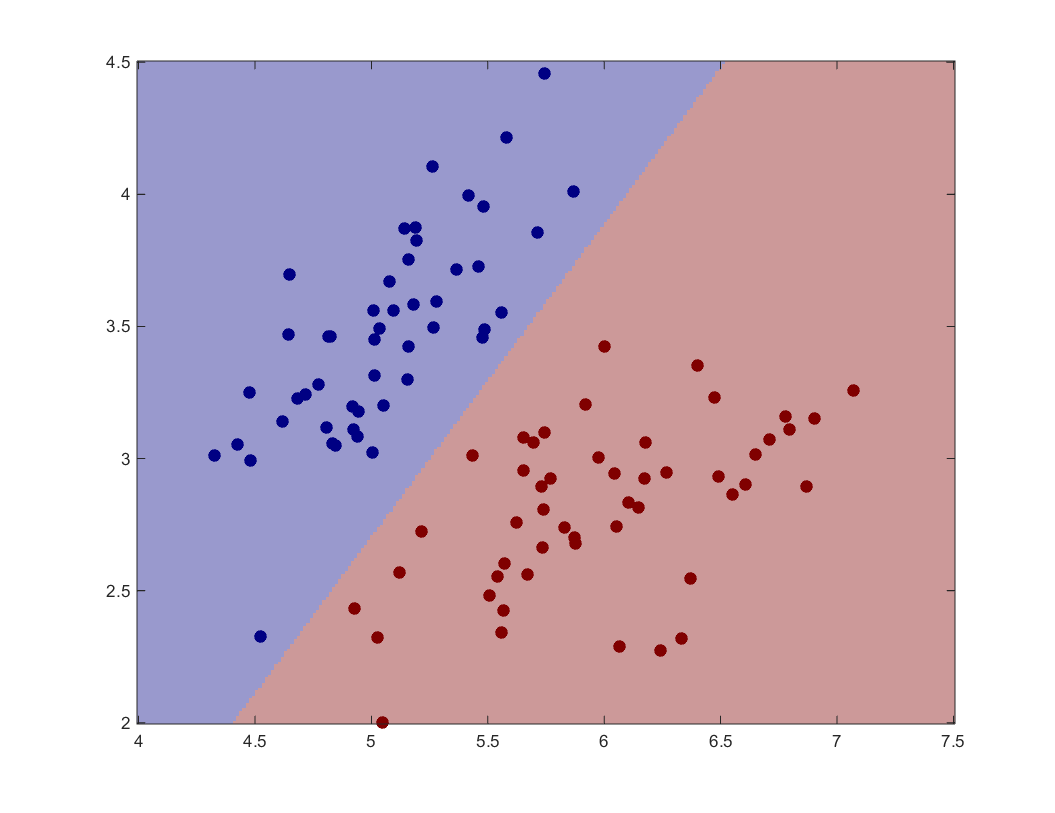
\includegraphics[width=6 in]{prob1Plot1.png}
\caption{Classification Plot with support vectors starred in yellow}
\end{figure}
\newpage
Here is the code to obtain the previous plot. The details of how I transformed into a version compatible with quadprog are in the comments. 
\lstinputlisting[firstline=1, lastline=49]{prob1.m}

\newpage

This is the code to obtain $\alpha$, verify it, and then plot the classification bounday. 
\lstinputlisting[firstline=51, lastline=119]{prob1.m}

\newpage

\section*{Problem 2}

\subsection*{Part a}

To calculate the entropy, I did the following
\[
H(y) = p(y=1)log_2(\frac{1}{p(y=1)}) + p(y=-1)log_2(\frac{1}{p(y=-1)})
\]
The entropy ends up being $0.9743$
\\

\subsection*{Part b}

You should split on feature 2 first. Here is the information gain for all the variables:\\
\\
\begin{tabular}{ c | c }
  Feature & Information Gain\\
  \hline                       
  1 & 0.0245 \\
  2 & 0.5059 \\
  3 & -0.0097 \\
  4 & 0.0930 \\
  5 & -0.0095 \\      
\end{tabular}

\newpage

\subsection*{Code for a and b}

This is the code to complete Part A and B. The code for the getEntropy function will be shown later.

\lstinputlisting[firstline=1, lastline=48]{prob2.m}

\subsection*{Part C}

Here is the decision tree for Part C

\begin{figure}[h]
\centering

\includegraphics[width=6 in]{hw4prob2DecisionTree.png}
\caption{Decision Tree}
\end{figure}

\newpage

Here is the code used in Part C. It relies on the data set up from Part A.

\lstinputlisting[firstline=50, lastline=82]{prob2.m}

\subsection*{Matlab functions written for Problem 2}

This is the code for the getEntropy function
\lstinputlisting[firstline=1, lastline=15]{getEntropy.m}

This is the code for the getDecTreeSplit function
\lstinputlisting[firstline=1, lastline=52]{getDecTreeSplit.m}
\end{document}
